\section*{Uma Primeira Se��o para o Ap�ndice}
\justifying
A matriz de Dilema Linear $M$ e o vetor de torques inerciais $b$,
utilizados na simula��o s�o calculados segundo a formula��o 
abaixo:

\begin{equation}
M=\left[ \begin{array}{ccc}
M_{11} & M_{12} & M_{13} \\
M_{21} & M_{22} & M_{23} \\
M_{31} & M_{32} & M_{33}
\end{array} \right]
\end{equation}

\begin{figure}[h]
\centering
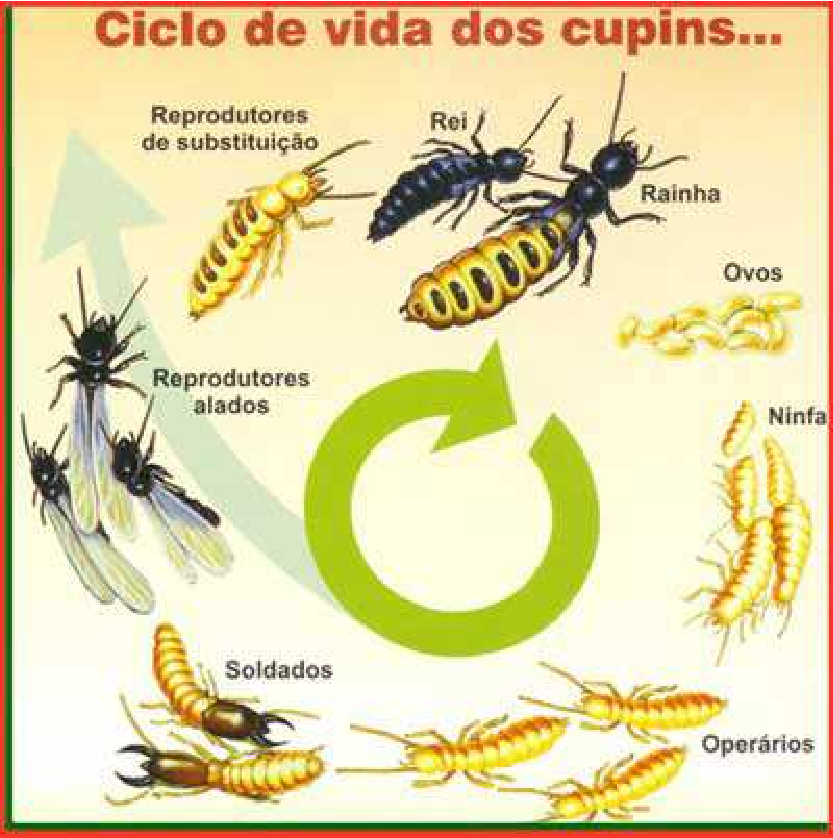
\includegraphics[height=5cm, width=5cm]{ApeA/pragas_ciclo_cupim}
\caption{Uma figura que est� no ap�ndice}\label{FD}
\end{figure}
